% LTeX: language=sl-SI
\section{Kriptografske osnove}
\label{sec:osnove}
Preden si lahko natančneje pogledamo, kako lahko skupina ustvari en sam podpis sporočila, si moramo 
pogledati nekaj kriptografskih osnov. Namen tega poglavja je predstaviti stvari, ki so predpogoj za
branje praktično kakršnegakoli kriptografskega besedila s področja digitalnih podpisov.

\subsection{Aritmetika v \texorpdfstring{$\Z_p^*$}{Zp∗}}
V kriptografiji imamo pogosto opravka z multiplikativnimi grupami, najenostavnejša med njimi (in
tudi tradicionalno največ uporabljena) je \textit{multiplikativna grupa naravnih števil modulo $p$},
ki jo označimo $\Z_p^*$. Njeni elementi so števila v $\{0, 1, \dots, p - 1\}$, ki so tuja številu $p$.
V posebnem primeru, ko je $p$ praštevilo, so to torej števila $\{1, 2, \dots, p - 1\}$ in je red grupe
(število elementov) $\text{ord}(\Z_p^*) = |\Z_p^*| = p - 1$. Operacija v tej grupi je, kot ime že
nakazuje, množenje modulo $p$.

Spomnimo se, da je red elementa $g$ v poljubni grupi najmanjše naravno število $q$, da velja $g^q = 1$,
kjer je $1$ enota za množenje. V primeru, da je $p$ praštevilo, je grupa $\Z_p^*$ \textit{ciklična},
kar pomeni, da v njej obstaja element $g$, katerega red je enak redu grupe, torej $\text{ord}(g) = p - 1$.
V tem primeru se $g$ imenuje \textit{generator}.

\begin{primer}[Grupa $\Z_{11}^*$]
\label{primer:Z11}
Ker je $11$ praštevilo, v grupi $\Z_{11}^*$ obstaja generator, oz.\ je grupa ciklična z redom $10 = 
11 - 1$. Z zaporednim računanjem potenc lahko vidimo, da je $\text{ord}(2) = 10$, torej je $2$ 
generator.

\begin{minipage}{0.45\textwidth}
    \begin{align*}
        2^1 &\equiv 2 \pmod{11} \\
        2^2 &\equiv 4 \pmod{11} \\
        2^3 &\equiv 8 \pmod{11} \\
        2^4 &\equiv 5 \pmod{11} \\
        2^5 &\equiv 10 \pmod{11} 
    \end{align*}
\end{minipage}
\begin{minipage}{0.45\textwidth}
    \begin{align*}
        2^6 &\equiv 9 \pmod{11} \\
        2^7 &\equiv 7 \pmod{11} \\
        2^8 &\equiv 3 \pmod{11} \\
        2^9 &\equiv 6 \pmod{11} \\
        2^{10} &\equiv 1 \pmod{11} 
    \end{align*}
\end{minipage}

\end{primer}

\begin{opomba}
    Spomnimo se \textit{kongruence}: $a \equiv b \pmod m \iff m \text{ }|\text{ } a - b$.
\end{opomba}

Za konec tega podpoglavja si oglejmo še nekaj trditev, ki bodo pomembne pri dokazovanju pravilnega
delovanja Schnorrovega podpisa.

\begin{trditev}
\label{trd:mod-q}
    Naj bosta $p$ in $q$ praštevili, kjer $q$ deli $p - 1$. Naj bo $g$ element grupe $\Z_p^*$ reda
    $q$, kar pomeni, da je $g^q \equiv 1 \pmod p$. Naj bo $k$
    naravno število. Potem velja 
    $$ 
    g^k \bmod p = g^{k \bmod q} \bmod p.
    $$
\end{trditev}
\begin{dokaz}
    Po osnovnem izreku o deljenju naravnih števil lahko $k$ na en sam način zapišemo kot $k = nq + r$, 
    kjer velja $n \in \N, r < q$.

    Leva stran enačbe se potem prepiše 
    \begin{align*}
        g^k \bmod p &= g^{nq + r} \bmod p = \\
                    &= (g^q)^n g^r \bmod p = \\
                    &= 1^n g^r \bmod p = \\
                    &= g^r \bmod p,
    \end{align*}
    kjer smo pri prehodu na tretjo vrstico upoštevali, da velja $g^q \equiv 1 \pmod p$. Desno stran
    pa lahko preoblikujemo na naslednji način:
    \begin{align*}
        g^{k \bmod q} \bmod p &= g^{(nq + r) \bmod q} \bmod p = \\ 
                              &= g^r \bmod p.
    \end{align*}
    Ker sta obe strani enaki, je trditev dokazana.
\end{dokaz}

\begin{trditev}
\label{trd:mod-mn-pt}
    Naj bodo $a$, $b$ in $p$ naravna števila. Potem za modularno množenje in potenciranje velja
    \begin{align}
        a \cdot b \bmod p &= (a \bmod p) \cdot (b \bmod p) \bmod p, \label{eq:mod-prod} \\
        a^b \bmod p &= (a \bmod p)^b \bmod p. \label{eq:mod-exp} 
    \end{align}
\end{trditev}
\begin{dokaz}
    Uporabimo osnovni izrek o deljenju naravnih števil, da $a$ in $b$ en sam način zapišemo kot 
    \begin{align*}
        a &= n_a p + r_a, \\
        b &= n_b p + r_b,
    \end{align*}
    kjer velja $r_a < p$ in $r_b < p$.

    \eqref{eq:mod-prod}: Levo stran preoblikujemo
    \begin{align*}
        a \cdot b \bmod p &= (n_a p + r_a) \cdot (n_b p + r_b) \bmod p = \\
                          &= (n_a n_b p^2 + n_a p r_b + n_b p r_a + r_a r_b) \bmod p = \\
                          &= r_a r_b \bmod p,
    \end{align*}
    desno pa
    \begin{align*}
        (a \bmod p) \cdot (b \bmod p) \bmod p &= (n_a p + r_a \bmod p) \cdot (n_b p + r_b \bmod p) \bmod p = \\
                          &= r_a r_b \bmod p.
    \end{align*}
    Ker se strani ujemata, je trditev dokazana.

    \eqref{eq:mod-exp}: Ker je potenciranje samo zaporedna uporaba množenj, lahko trditev pokažemo z 
    indukcijo na $b$ in enačbo~\eqref{eq:mod-prod}:
    \begin{itemize}
        \item $b = 2$: Primer, ko je $b = 1$ (ali $b = 0$) je trivialen, če pa je $b = 2$, pa se 
            problem reducira v 
            $$ 
            a \cdot a \bmod p \stackrel{?}{=} (a \bmod p) \cdot (a \bmod p) \bmod p,
            $$
            kar drži neposredno po enačbi~\eqref{eq:mod-prod}.
        \item $n \rightarrow n + 1$: Predpostavimo, da enačba~\eqref{eq:mod-exp} drži za $b = n$ (I.P.). 
            Ko je $b = n + 1$, dobimo 
            \begin{align*}
                a^{n + 1} \bmod p &= a^n a \bmod p = \\ 
                                  &\stackrel{\eqref{eq:mod-prod}}{=} (a^n \bmod p) (a \bmod p) \bmod p = \\
                                  &\stackrel{\text{I.P.}}{=} (a \bmod p)^n (a \bmod p) \bmod p = \\
                                  &= (a \bmod p)^{n + 1} \bmod p.
            \end{align*}
    \end{itemize}
    S tem je indukcija končana in trditev dokazana.
\end{dokaz}

\begin{trditev}
\label{trd:exp-mod-ord}
    Naj bo $G$ končna ciklična grupa reda $q$ z generatorjem $g$. Naj bo $n$ poljubno naravno število.
    Potem velja
    $$
    g^n = g^{n \bmod q}.
    $$
\end{trditev}
\begin{dokaz}
    Po definiciji reda elementa grupe in generatorja grupe velja, da je
    $$
    g^q = 1.
    $$
    Po osnovnem izreku o deljenju naravnih števil lahko $n$ na en sam način zapišemo kot $n = mq + r$,
    kjer velja $m \in \N$ in $0 \leq r < q$. Potem lahko zapišemo
    $$
    g^n = g^{mq + r} = (g^q)^m g^r = 1^m g^r = g^{mq + r \bmod q} = g^{n \bmod q}.
    $$
\end{dokaz}

\subsection{Zgoščevalne funkcije}
V grobem so (kriptografske) \textit{zgoščevalne funkcije} take funkcije, ki prejmejo poljubno dolg binarni
niz (ki lahko predstavlja besede, številke, celotne dokumente, \dots), vrnejo pa binarni niz, ki ima
vnaprej določeno dolžino. Tem rezultatom pravimo \textit{zgostitve}. Namen zgoščevalnih funkcij je
za dokument ustvariti kratek niz, ki unikatno identificira dokument. Želimo si, da je v praksi
nemogoče najti dva različna niza z enako zgostitvijo. Natančno zgoščevalne funkcije definiramo:

\begin{definicija}
\label{def:hash}
    \textbf{Kriptografska zgoščevalna funkcija} $H: \{0, 1\}^* \rightarrow \{0, 1\}^n$ je funkcija, 
    ki slika binarne nize $m$ poljubne dolžine v njihove \textbf{zgostitve} $H(m)$, tj.\ binarne nize 
    vnaprej določene dolžine $n$. Zadoščati mora naslednjim lastnostim:
    \begin{itemize}
        \item \textbf{Določenost} pomeni, da bo zgoščevanje enakih nizov vedno privedlo do enake 
            zgostitve, tj.\ $H$ je funkcija in ne naključni algoritem. Zapišemo lahko
            $\forall m: ((h_1 = H(m) \wedge h_2 = H(m)) \implies h_1 = h_2)$.
        \item \textbf{Učinkovitost} pomeni, da lahko računalnik izračuna poljubno zgostitev v doglednem 
            času. Izračun zgostitve mora biti računsko učinkovit. Običajno tu zahtevamo, da je časovna
            zahtevnost funkcije $H$ polinomska v dolžini vhodnega niza.
        \item \textbf{Enosmernost} oz.\ \textbf{odpornost na prasliko} pomeni, da iz predložene 
            zgostitve zelo težko ugotovimo, kateri niz je funkcija prejela kot vhod. Če torej poznamo 
            zgostitev $h$ za nek neznan $m$, je računsko neizvedljivo najti niz $m$, da velja $h = H(m)$.
        \item \textbf{Odpornost na drugo prasliko} pomeni, da če poznamo niz in njegovo zgostitev, 
            zelo težko najdemo drug niz z enako zgostitvijo. Če torej poznamo niz $m_1$ z zgostitvijo
            $h_1$, je računsko neizvedljivo najti zgostitev $m_2$, da velja $H(m_2) = h_1$.
        \item \textbf{Odpornost na trke} pomeni, da je računsko neizvedljivo najti dva niza $m_1$
            in $m_2$, ki imata enako zgostitev, oz.,\ da velja $H(m_1) = H(m_2)$.
        \item \textbf{Učinek plazu} pomeni, da vsaka sprememba v vhodnem nizu povzroči veliko in
            nepredvidljivo spremembo v zgostitvi. Če spremenimo en bit v vhodnem nizu, v povprečju
            pričakujemo, da se spremeni polovica bitov v zgostitvi.
    \end{itemize}
\end{definicija}

\begin{opomba}
    Vse varne kriptografske zgoščevalne funkcije, ki so v uporabi zadoščajo zgornjim lastnostim. To
    pomeni, da za nobeno od teh funkcij nihče še ni našel trka.
\end{opomba}

\begin{primer}
    Ena izmed najbolj znanih zgoščevalnih funkcij je \texttt{SHA-256}. Njeno ime pomeni \textit{Secure
    Hash Algorithm} (slov.\ varen zgoščevalni algoritem), $256$ pa predstavlja dolžino vrnjene zgostitve.
    Pogostokrat to ime zasledimo pri nameščanju programske opreme, kjer služi kot avtentikator, da smo res
    naložili pravi program. Preverja namreč, da se zgostitvi naloženih in prenešenih datotek ujemajo.

    Za primer si lahko ogledamo zgostitvi dveh podobnih nizov, \textit{Ljubljana} in \textit{Ljubljena}. 
    Kljub podobnosti bomo videli, da sta rezultata popolnoma drugačna, kar si tudi želimo pri zgoščevalnih 
    funkcijah.
    \begin{verbatim}
    SHA-256(Ljubljana) =
    b7f147d8b4a6703a951336654355071f9752385f85d0860379e99b484aee7a82

    SHA-256(Ljubljena) =
    995d2d8ffb40e1838219e65dd2c665701ba34a90e11f7195a4b791838b6787fe
    \end{verbatim}
    Za preglednost nismo prevajali besed v binarne nize, to bi storili npr.\ z \texttt{ASCII} ali \texttt{UTF-8}
    tabelo. Prav tako smo rezultat napisali v šestnajstiškem sistemu, saj je tako krajši. Iz rezultatov
    pa nazorno vidimo učinek plazu, saj sta popolnoma drugačna.
\end{primer}

\subsection{Kriptografija javnega ključa}
Prve šifre, ki smo jih uporabljali ljudje, so bile \textit{simetrične}, kar pomeni, da sta osebi
za komunikacijo obe morali poznati skriven \textit{ključ}, s pomočjo katerega sta tako ustvarjali
šifre, kot jih tudi dešifrirali. Ključ je običajno neko dolgo (binarno) število.

\begin{primer}[Cezarjeva šifra]
    Ena najbolj znanih šifer, ki izvira iz Antičnega Rima, je \textit{Cezarjeva šifra}. Njen ključ 
    je število, ki je krajše od dolžine naše abecede, v Cezarjevem primeru je bilo to število $3$.
    Šifra potem deluje tako, da vsako črko zamakne za toliko mest v abecedi, kolikor definira 
    ključ. Npr.\ za slovensko abecedo, bi šifra zamaknila črke:
    \begin{verbatim}
        A B C Č D E F G H I J K L M N O P R S Š T U V Z Ž
        Č D E F G H I J K L M N O P R S Š T U V Z Ž A B C
    \end{verbatim}
    To bi izraz \texttt{JAVNI KLJUČ} preslikalo v \texttt{MČARL NOMŽF}. Cezarjeva šifra se imenuje 
    tudi \textit{zamična šifra}.
\end{primer}

V prejšnjem stoletju pa se je pojavila alternativa, imenovana \textit{asimetrična kriptografija}, oz.\
\textit{kriptografija javnega ključa}. Glavna prednost te je, da osebi za komunikacijo ne rabita
poznati enakega skrivnega ključa, vendar ima vsak od njiju par ključev, ki ju imenujemo \textbf{javni
ključ} (angl.\ \textit{public key}) in \textbf{zasebni ključ} (angl.\ \textit{secret/private key}) in
označimo kot par $(\text{pk}, \text{sk})$. Vsaka oseba objavi svoj javni ključ in poskrbi, da nihče 
ne izve, kaj je njen zasebni ključ.

Šifriranje potem poteka tako, da pridobimo javni ključ od osebe, s katero želimo komunicirati, ga
uporabimo za šifriranje in objavimo šifrirano sporočilo. Lastnik ustreznega zasebnega ključa (vsakemu
javnemu pripada natanko en zasebni) potem pridobi šifrirano sporočilo in ga z zasebnim ključem
dešifrira. Kriptosistemi delujejo na način, da lahko sporočilo, šifrirano z javnim ključem dešifrira
samo ustrezen zasebni ključ. Tako zagotovimo varno komunikacijo.

\begin{primer}[RSA]
\label{primer:rsa}
    En prvih algoritmov javnega ključa, ki se uporablja še danes, je \textit{RSA}. Njegova varnost izhaja 
    iz (domnevne) težavnosti problema iskanja prafaktorjev velikega števila. Svoj ključ definiramo tako, 
    da si izberemo dve (zelo veliki) praštevili $p$ in $q$, ter ju zmnožimo v $n = pq$. Za primer vzemimo 
    $p = 23$ in  $q = 17$. $n$ je potem enak $391$. Izbrati si moramo še eksponent $e$, vzemimo npr. $e = 3$. 
    Naš javni ključ je potem par 
    $$ 
    (n, e) = (391, 3).
    $$
    Postopek šifriranja poteka tako, da oseba, s katero komuniciramo, izbere sporočilo $m$, npr.\ 
    $m = 10$, pridobi naš javni ključ, in izračuna šifro $c$ kot
    $$
    c = m^e \bmod{n} = 10^3 \bmod{n} = 218.
    $$
    Dogovoriti se moramo še o zasebnem ključu. Za to bomo potrebovali eksponent za dešifriranje $d$,
    tako da bo veljalo 
    $$
    (m^e)^d \equiv 1 \pmod{\varphi(n)},
    $$ 
    kjer $\varphi$ označuje Eulerjevo funkcijo. Iščemo torej multiplikativni inverz eksponenta 
    $e$, modulo $\varphi(n)$. V našem primeru je to $d = 235$. Zasebni ključ je potem 
    $$ 
    (p, q, d) = (23, 17, 235). 
    $$
    Iz zasebnega ključa torej lahko kadarkoli izračunamo javnega, saj enostavno zmnožimo $p$ in $q$ 
    ter izračunamo inverz, v splošnem pa iz $n$ učinkovito ne moremo pridobiti faktorjev $p$ in $q$,
    kar nam zagotavlja varnost.

    Ko prejmemo šifrirano sporočilo $c$, ga dešifriramo tako, da izračunamo
    $$
    m = c^d \bmod{n} = 218^{235} \bmod{391} = 10.
    $$
\end{primer}

Poleg šifriranja, brez da bi si delili ključ, pa je kriptografija javnega ključa omogočila tudi
\textit{digitalne podpise}. Ti so uporabljeni vsakič, ko pošljemo transakcijo ali dostopamo do katerekoli
spletne strani. Delujejo na podoben način kot šifriranje z javnim ključem, le da najprej uporabimo
zasebni ključ na sporočilu, prek javnega ključa pa preverjamo veljavnost podpisa. Velikokrat sta šifrianje
in podpisovanje uporabljena hkrati, saj tako pošljemo šifrirano sporočilo, ki ga lahko prebere le oseba,
kateri je namenjeno, hkrati pa lahko preveri, da je res prišlo od nas.

\subsection{Digitalni podpisi}
Ideja \textit{kriptografskih} ali \textit{digitalnih podpisov} (angl.\ \textit{digital signatures}) je,
da služijo kot izboljšava človeškega ročnega podpisa. Za razliko od ročnega podpisa, lahko z digitalnim
dosežemo pravo identifikacijo posameznika, ki temelji na njegovem zasebnem ključu. Tako smo lahko
za digitalno podpisan dokument prepričani, da ga je res podpisal lastnik točno določenega zasebnega ključa
(če predpostavimo, da podpisnik ključa ni posredoval nikomur).

Podpis dokumenta poteka nekoliko drugače, kot pri ročnih podpisih. Pri ročnem podpisu ta postane del
dokumenta, digitalni podpis pa je od njega ločen, vseeno pa nastane s pomočjo zgostitve podpisanega
dokumenta. Zato bo podpis za dva različna dokumenta vedno drugačen (dokler uporabimo varno zgoščevalno
funkcijo).

Ostane še vprašanje preverjanja avtentičnosti podpisa. Pri ročnem podpisu to lahko storimo prek 
primerjave z znanim, preverjeno avtentičnim podpisom. Ta postopek je zamuden in nenatančen, veliko 
večino ročnih podpisov je moč ponarediti z nekaj prakse. Preverjanje digitalnega podpisa pa temelji 
na kriptografiji javnega ključa. Ker je podpis nastal s pomočjo podpisnikovega zasebnega ključa,
lahko s pomočjo ujemajočega javnega ključa preverimo avtentičnost.

Da se lažje pogovarjamo o kriptografskih sistemih, je smotrno definirati, kaj točno so deležniki,
kot so podpisnik, preverjevalec in napadalec. V kriptografskih besedilih so pogosto definirani kot
verjetnostni Turingovi stroji, mi pa se bomo izognili tej formalizaciji in se pogovarjali enostavno
o \textit{naključnostnih algoritmih}. Te lahko definiramo kot navadne, deterministične algoritme,
ki imajo dostop do dodatnega parametra, \textit{vira naključnih bitov} $\omega$. Ta vir si lahko
predstavljamo kot zelo dolg seznam naključnih bitov, ki ga algoritem lahko bere, ko ga potrebuje
(npr.\ za generiranje naključnih števil). Branje je ponavadi enkratno dejanje; ko algoritem prebere
bit, mora pri naslednjem klicu prebrati naslednji bit.

\begin{definicija}
\label{def:digisig}
    \textbf{Digitalni} ali \textbf{kriptografski podpis} $\mathcal{S} = (\mathcal{P}, \mathcal{G},
    \mathcal{S}, \mathcal{V})$ je četvorka učinkovitih algoritmov $\mathcal{P}$ za ustvarjanje parametrov
    podpisa, $\mathcal{G}$ za ustvarjanje ključa, $\mathcal{S}$ za podpisovanje in $\mathcal{V}$ za
    preverjanje podpisa. Definirana je nad končno množico možnih  sporočil $\mathcal{M}$, vrnjeni
    podpis pa leži v končni množici podpisov $\Sigma$.
    \begin{itemize}
        \item $\mathcal{P}$ je algoritem za ustvarjanje javnih parametrov podpisa. Definira množico
            parametrov $\text{Par}$, ki so na voljo vsem deležnikom pri podpisu. V praksi je ta korak izpuščen,
            sodelujoči pri podpisu si izberejo shemo in uporabijo dobro poznane varne parametre.
            Formalno pa je to algoritem, ki prejme varnostni parameter $k$ in vrne parametre
            $\text{Par}$, oz.\
            $$
            \text{Par} = \mathcal{P}(k).
            $$
        \item $\mathcal{G}$ je naključnostni algoritem za ustvarjanje para ključev $(\text{pk}, \text{sk})$, 
            ki za svoj vhod prejme parametre $\text{Par}$ (javno dostopni ali pa ustvarjeni prek $\mathcal{P}$).
            Z javnim ključem $\text{pk}$ lahko preverjevalec preveri avtentičnost podpisa, z zasebnim
            ključem $\text{sk}$ pa podpisnik podpisuje. Formalno velja
            $$
            (\text{pk}, \text{sk}) = \mathcal{G}(\text{Par}).
            $$
        \item $\mathcal{S}$ je naključnostni algoritem, ki za svoja argumenta prejme zasebni ključ $\text{sk}$
            in sporočilo $m$, vrne pa podpis $\sigma$ sporočila $m$ z zasebnim ključem $\text{sk}$
            oz.\
            $$
            \sigma = \mathcal{S}(\text{sk}, m).
            $$
        \item $\mathcal{V}$ je determinističen algoritem, ki preverja veljavnost podpisov. Za svoje argumente
            prejme javni ključ $\text{pk}$, sporočilo $m$ in podpis $\sigma$, vrne $veljaven$, če je podpis 
            veljaven, in $neveljaven$, sicer. Velja torej
            $$ 
            \mathcal{V}(\text{pk}, m, \sigma) =
            \begin{cases}
                veljaven, & \text{podpis veljaven}, \\
                neveljaven, & \text{sicer}.
            \end{cases}
            $$
            Podpis $\sigma$ sporočila $m$ je veljaven, če je bil ustvarjen z uporabo algoritma
            $\mathcal{S}$ in zasebnim ključem $\text{sk}$, ki ustreza javnemu ključu $\text{pk}$.
    \end{itemize}
\end{definicija}

\begin{primer}
    Digitalni podpisi, obravnavni v tem besedilu, temeljijo na grupah. Algoritem $\mathcal{P}$ iz
    definicije~\ref{def:digisig} v tem primeru izbere parametre, ki določajo grupo $G$. Za varnostni
    parameter $k$ lahko zapišemo 
    $$
    G = \mathcal{P}(k).
    $$
\end{primer}

\subsection{Varnost}
Poglavitna lastnost vsakega kriptosistema je njegova \textit{varnost}. Ker je namen digitalnih podpisov
zagotoviti sogovorniku, da je sporočilo res poslal lastnik zasebnega ključa, je največja varnostna
skrb, da bi \textit{napadalec} lahko ponaredil pošiljateljev podpis in si s tem prisvojil njegovo
identiteto. To napadalcu lahko uspe na več nivojih, ki jih lahko razvrstimo od najmanj do najbolj
škodljivega:

\begin{itemize}
    \item \textbf{Eksistencialno ponarejanje} (angl.\ \textit{existential forgery}) pomeni, da obstaja
        sporočilo, za katerega napadalec lahko ustvari ponarejen podpis (torej podpis, pri katerem
        ni bil uporabljen zasebni ključ). To pomeni, da lahko najde vsaj en par sporočila in podpisa
        $(m, \sigma)$, da velja $\mathcal{V}(\text{pk}, m, \sigma) = veljaven$.
    \item \textbf{Selektivno ponarejanje} (angl.\ \textit{selective forgery}) pomeni, da lahko napadalec
        z nezanemarljivo verjetnostjo podpiše poljubno izbrano sporočilo, ki ga lastnik zasebnega
        ključa še ni podpisal. Torej, če napadalcu nekdo predloži sporočilo $m$, lahko z nezanemarljivo
        verjetnostjo najde podpis $\sigma$, da velja $\mathcal{V}(\text{pk}, m, \sigma) = veljaven$.
    \item \textbf{Popoln zlom} (angl.\ \textit{total break}) pomeni, da napadalec pridobi
        zasebni ključ napadenega in s tem pridobi vse potrebne podatke za podpisovanje poljubnih
        sporočil v njegovem imenu.
\end{itemize}

Poleg zgoraj definiranih \textit{ciljev napadalca}, lahko za vsak kriptosistem definiramo tudi
\textit{model napada}, ki ga zagotavlja shema. Stinson~\cite{stinson2023crypto} definira naslednje
modele:
\begin{itemize}
    \item \textbf{Napad samo s ključem} je napad, kjer napadalec pozna javni ključ žrtve $\text{pk}$. 
        Predpostavimo tudi, da napadalec vedno pozna delovanje sheme za podpisovanje $\mathcal{S}$
        in ima dostop do javnih parametrov podpisa $G$. Z javnim ključem torej lahko preverja
        veljavnost podpisov, ni pa prejel nobenega podpisanega sporočila.
    \item \textbf{Napad z znanimi sporočili} je napad, kjer napadalec poseduje seznam parov sporočil 
        in njihovih podpisov $(m_1, \sigma_1), (m_2, \sigma_2), \dots$, kjer za vsak $i$ velja 
        $\sigma_i = \mathcal{S}(\text{sk}, m_i)$.
    \item \textbf{Napad z izbranimi sporočili} je napad, kjer napadalec podpisniku da seznam sporočil $m_1,
        m_2, \dots$, ta pa mu vrne seznam podpisov, da za vsak $i$ velja $\sigma_i = \mathcal{S}(\text{sk}, 
        m_i)$. Napadalčev cilj je iz predloženih parov izvleči zasebni ključ, ali pa na nek drug način
        podpisati še ne podpisano sporočilo.
\end{itemize}

Ostane nam še pregled \textit{tipov varnosti}, ki jo lahko pričakujemo oz.\ zahtevamo od sheme za
podpisovanje. Takšna shema ne more biti \textit{brezpogojno varna}, kar bi pomenilo, da je tudi z
neomejenimi računskimi zmožnostmi nemogoče ponarediti podpis. To je zato, ker lahko napadalec
sistematično preveri vse podpise za neko sporočilo s pomočjo algoritma $\mathcal{V}$, dokler ne najde
pravega. Pričakujemo pa lahko \textit{računsko varnost}, kar pomeni, da napadalec ne more najti
ponaredka v doglednem času, če ima omejene računske sposobnosti, oziroma \textit{dokazljivo varnost},
kar pomeni, da lahko varnost prevedemo na težavnost nekega matematičnega problema. Varnost večine
shem za digitalne podpise temelji prav na (domnevni) težavnosti določenih matematičnih problemov.

\subsubsection{Temelji varnosti}
V primeru~\ref{primer:rsa} smo omenili, da je varnost algoritma RSA odvisna od težavnosti problema
iskanja prafaktorjev velikega števila. To je le eden izmed mnogih problemov, ki služijo kot osnova
za varnost kriptografskih sistemov. V kriptografiji javnega ključa se pogosto srečamo s cikličnimi
grupami, ki podpirajo množenje. V nadaljevanju bomo pogosto uporabili operacijo množenja, za izračune
tipa 
$$
I = g^s,
$$
kjer je $g$ generator ciklične grupe, $s$ pa zasebni ključ. Zaradi notacije bi morda kdo hitro pomislil,
da lahko zgornjo enačbo obrnemo in $s$ izračunamo kot 
$$ 
s = \log_g(I).
$$
Taki izračuni v (nekaterih) cikličnih grupah žal (ali pa na srečo) niso tako enostavni, prišli smo do
koncepta \textit{diskretnega logaritma}. Pri izračunu logaritmov v množici realnih števil ključno
vlogo igra koncept urejenosti. Ker je eksponentna funkcija strogo naraščajoča, realna števila pa urejena,
lahko učinkovito izračunamo logaritme do poljubne natančosti (npr.\ z uporabo bisekcije). V diskretnih
cikličih grupah, kot je npr.\ $\Z_p^*$, ni koncepta urejenosti, kar smo videli tudi v
primeru~\ref{primer:Z11} z grupo $\Z_{11}^*$. Odnos med $g^s_1$ in $g^s_2$ nam ne pove ničesar o
odnosu med $s_1$ in $s_2$, zato nam ">približki"< logaritma ne pomagajo čisto nič. Za izračun takih
logaritmov se moramo zanesti na drugačne metode, kot za izračun logaritmov v množici realnih števil.

\begin{definicija}[Problem diskretnega logaritma~\cite{boneh2023appcry}]
\label{def:dl}
    Naj bo $G$ ciklična grupa reda $q$, ki jo generira element $g$. Naj bo $h$ naključni element iz 
    grupe $G$. Naj velja $g^x = h$. Eksponent $x$ imenujemo \textbf{Diskretni logaritem (DL)}.

    Zamislimo si igro, kjer izzivalec in nasprotnik kot vhod prejmeta opis grupe $G$ (torej $q \in \N$
    in $g \in G$). Izzivalec potem izbere naključen element $\alpha \in G$ in izračuna $h = g^{\alpha}$.
    $h$ pošlje nasprotniku, ta pa mora odgovoriti nazaj z elementom $\alpha$. To igro imenujemo 
    \textbf{problem diskretnega logaritma (PDL)} (angl.\ \textit{discrete logarithm problem}).

    Pri tej igri nas zanima verjetnost pravilnega odgovora nasprotnika, ki je računsko omejen. S tem
    mislimo, da ima na voljo polinomsko mnogo časa (glede na število bitov $q$). Če je grupa $G$ takšna,
    da je verjetnost zanemarljiva, pravimo, da za grupo $G$ drži \textit{predpostavka o težavnosti
    diskretnega logaritma}.
\end{definicija}

Če naš kriptosistem torej živi v ciklični grupi, v kateri je problem diskretnega logaritma težek,
nam to zagotavlja, da iz javnega ključa ni računsko izvedljivo pridobiti zasebnega. To je osnova
za varnost mnogih kriptografskih sistemov, kot sta npr.\ ElGamalov sistem~\cite{elgamal1985elgamal}
in Schnorrov podpis~\cite{schnorr1989sig}.

Preden nadaljujemo, natančneje definirajmo, kaj pomeni, da je verjetnost zanemarljiva.

\begin{definicija}[Zanemarljiva funkcija~\cite{boneh2023appcry}]
    Zanemarljiva funkcija je taka funkcija $\varepsilon : \N \rightarrow \R$, da za vsako število
    $c > 0$ obstaja naravno število $n_0 \in \N$, da za vsak $n > n_0$ velja
    $$
    |\varepsilon(n)| < \frac{1}{n^c}.
    $$
    V nadaljevanju bomo v $\varepsilon$ označevali poljubno zanemaljivo funkcijo.
\end{definicija}

To so torej funkcije, ki padajo proti nič hitreje, kot inverz kateregakoli polinoma. V kontekstu
diskretnega logaritma želimo, da je verjetnost izračuna pravilnega odgovora nasprotnika zanemarljiva.

V besedilu bomo večkrat govorili o ">zanemarljivih verjetnostih"<, kar pomeni, da se bodo
verjetnosti v odvisnosti od določene spremenljivke vedle kot zanemarljive funkcije.

\subsubsection{Model slučajnega oraklja}
Ko obravnavamo varnost kriptosistemov, se ponavadi pogovarjamo o \textit{standardnemu modelu} kriptografije.
Ta model ima samo eno predpostavko: napadalec je omejen samo s časom in količino računske moči, ki mu
je na voljo (tu je običajno predpostavljeno, da ima napadalec realno računsko moč). Občasno se znajdemo
v primeru, ko moramo za dokaz varnosti sprejeti dodatne predpostavke. V tem primeru govorimo o
alternativnih modelih kriptografije. 

Ko imamo opravka z zgoščevalnimi funkcijami, je pogosto potrebno sprejeti dodatne predpostavke, da lahko
pokažemo varnost. Specifično, ko imamo opravka z zgoščevalno funkcijo $H: A \rightarrow B$, predpostavimo,
da je bila ta funkcija izbrana naključno med vsemi funkcijami, ki slikajo $A$ v $B$. To idealizirano 
verzijo zgoščevalne funkcije imenujemo \textbf{slučajni orakelj} (angl.\ \textit{random oracle}).
Za poljuben vhod torej vedno vrne enak odgovor, vendar je bil ta odgovor popolnoma naključno izbran.

\textbf{Model slučajnega oraklja} (angl.\ \textit{random oracle model}) je model kriptografije, kjer poleg 
standardnih predpostavk, vsako uporabo zgoščevalne funkcije nadomestimo s slučajnim 
orakljem~\cite{boneh2023appcry}. Predpostavimo, da imajo do oraklja dostop vsi vpleteni v kriptosistem, 
vključno z napadalcem.

Varnostni dokazi, ki temeljijo na uporabi takih slučajnih orakljev, vseeno pričajo o varnosti shem,
ki namesto orakljev uporabljajo zgoščevalne funkcije, vsaj dokler je uporabljena zgoščevalna funkcija
varna (npr.\ zanjo nihče še ni našel trka).

\begin{opomba}
    V praksi imamo pogosto opravka z elementi grup in zgoščevalnimi funkcijami, ki slikajo en niz bitov
    v drugega. Zato je potrebno definirati funkcijo $\text{enc}: G \rightarrow \{0, 1\}^*$, ki slika
    elemente grupe $G$ v nize bitov. Prek te funkcije lahko pridobimo zgostitve poljubnih elementov grup.
\end{opomba}

\subsubsection{Dokazovanje varnosti}
Pogosto je cilj varnostnih dokazov pokazati, da je varnost neke sheme enakovredna težavnosti nekega
problema, za katerega domnevamo, da je težek. V takih primerih govorimo o metodi
\textit{dokazovanja z redukcijo} (angl.\ \textit{reduction proof}). Ta metoda temelji na predpostavki,
da če bi napadalec lahko učinkovito napadel shemo, bi lahko tudi učinkovito rešil težaven problem.

En način, kako to storimo, je z uporabo \textit{iger}. Potek dokaza varnosti v tem primeru je sledeč:
\begin{itemize}
    \item Naj bo $\mathcal{S}$ podpisna shema, za katero želimo pokazati varnost (npr.\ da je verjetnost
        ponarejanja zanemarljiva). To shemo napada napadalec $\mathcal{F}$, ki je omejen s
        polinomskim časom. Napadalčevi interakciji s podpisno shemo rečemo \textit{igra}, zanima
        pa nas verjetnost ">zmage"< napadalca, torej uspešnega ponarejenja podpisa.
    \item Definiramo še en algoritem $\mathcal{A}$. Cilj tega algoritma je izvesti redukcijo
        iz napada na reševanje težavnega problema. Algoritem $\mathcal{A}$ mora v polinomskem času
        prevesti uspešen napad napadalca $\mathcal{F}$ na shemo $\mathcal{S}$ v rešitev težavnega
        problema. Ponavadi to pomeni, da algoritem $\mathcal{A}$ sodeluje pri izvajanju podpisne sheme.
        Za dokaz analiziramo verjetnost uspeha algoritma $\mathcal{A}$, ki je seveda odvisna
        od verjetnosti uspeha napadalca $\mathcal{F}$.

        Navadno v dokazu predpostavimo, da je napadalec $\mathcal{F}$ uspešen z nezanemarljivo
        verjetnostjo, kar se prevede v nezanemarljivo verjetnost uspeha algoritma $\mathcal{A}$.
        Ker bi to pomenilo uspešno rešitev težavnega problema v polinomskem času, zaključimo, da je
        shema varna.
\end{itemize}

Za algoritem $\mathcal{A}$ predpostavimo naslednje lastnosti:
\begin{itemize}
    \item \textbf{Nerazločljivost}: Napadalec $\mathcal{F}$ ne ve, ali komunicira s pravim podpisnikom
        ali z algoritmom $\mathcal{A}$. Če bi lahko napadalec razlikoval, potem bi lahko zaključili,
        da shema napadalcu razkrije neko skrivnost, saj je prisotnost skrivnosti edina razlika med
        pravim podpisnikom in algoritmom $\mathcal{A}$.
    \item \textbf{Brez skrivnosti}: Algoritem $\mathcal{A}$ ne pozna zasebnih ključev. Ta lastnost
        je ključna, saj nam pove, da napadalec prek interakcije z dejanskim podpisnikom ne izve
        nobene dodatne informacije. Če je napadalec uspešen pri interakciji z algoritmom $\mathcal{A}$
        ali pa podpisnikom, ki ima zasebni ključ, potem smo lahko prepričani, da prisotnost zasebnega
        ključa ne pomaga pri napadu.
    \item \textbf{Prilagodljivost}: Algoritem $\mathcal{A}$ in napadalec med seboj komunicirata.
        Pogosto je potrebno, da algoritem $\mathcal{A}$ prilagodi svoje odločitve na podlagi
        napadalčevih odločitev.

        V modelu slučajnega oraklja prilagodljivost dobi dodatno dimenzijo. Algoritem $\mathcal{A}$
        poleg celotnega protokola simulira tudi delovanje oraklja. To mu omogoča, da napadalca ">previje"<
        na prejšnje stanje, prilagodi odgovor oraklja in ponovno izvede korak sheme.
\end{itemize}

\subsection{Interaktivni protokoli}
V tem razdelku bomo govorili o \textit{interaktivnih protokolih} (angl.\ \textit{interactive protocols}).
To so protokoli, kjer si dva sogovornika izmenjujeta sporočila, dokler ne prideta do skupnega zaključka.
Pogosto se uporabljajo za namene avtentikacije, kjer ena stran dokazuje svojo identiteto drugi.
Zaradi te uporabe, bomo sogovornika poimenovali \textit{dokazovalec} (angl.\ \textit{prover}) in
\textit{preverjevalec} (angl.\ \textit{verifier}). Taki protokoli so sorodni digitalnim podpisom,
pogosto pa so uporabljeni pri konstrukciji bolj zahtevnih kriptografskih shem.

Avtentikacijo lahko vidimo kot poseben primer dokazovanja. Dokazovalec želi dokazati preverjevalcu, da
je res tisti, za katerega se izdaja. Protokoli, kjer je cilj dokazati neko trditev, sodijo v skupino
\textit{interaktivnih sistemov dokazovanja} (angl.\ \textit{interactive proof systems}). Formalno
morajo taki protokoli zadoščati dvema lastnostma:
\begin{itemize}
    \item \textbf{Celovitost} (angl.\ \textit{completeness}): Če trditev, ki se dokazuje,
        drži, potem bo preverjevalec sprejel dokaz dokazovalca (če noben od njiju ne bo goljufal).
    \item \textbf{Zadostnost} (angl.\ \textit{soundness}): Če trditev, ki se dokazuje, ne
        drži, potem noben dokazovalec (tudi tak, ki goljufa) ne more predložiti dokaza, ki bi 
        ga preverjevalec sprejel, razen z zanemarljivo verjetnostjo.
\end{itemize}
Dejanski interaktivni protokol pa potem deluje kot izmenjava sporočil, kjer dokazovalec poskuša
prepričati preverjevalca, da trditev drži, preverjevalec pa s serijo vprašanj preverja, če je
dokazovalec iskren in če trditev res drži. Pogosto predpostavimo, da ima dokazovalec neomejeno
računsko moč, vendar ni iskren, preverjevalec pa je omejen na polinomsko računsko moč in je iskren.

\begin{primer}[Reševanje sudokuja]
    Za enostaven primer interaktivnega dokaza si oglejmo reševanje posplošenega Sudokuja. Tradicionalni
    Sudoku je problem, kjer moramo v $9 \times 9$ mrežo zapolniti števila od $1$ do $9$ tako, da se v vsaki
    vrstici, stolpcu in $3 \times 3$ kvadratu ne ponovijo nobena števila. Problem posplošimo tako, da
    ga prenesemo na poljubno mrežo velikosti $n^2 \times n^2$ in dovolimo uporabo števil od $1$ do $n^2$.

    Znano je, da je ta problem NP-poln~\cite{yato2003sudoku}, kar pomeni, da je težko najti rešitev,
    vendar je enostavno preveriti, če je rešitev pravilna. Če želi dokazovalec prepričati preverjevalca,
    da zna rešiti vse Sudokuje, lahko to storita tako, da si preverjevalec izbere naključne Sudokuje,
    jih pošlje dokazovalcu, ta pa jih reši in vrne rešitve. Preverjevalec nato preveri, če so rešitve pravilne.
    Po dovolj velikem številu preverjenih Sudokujev, bo preverjevalec lahko prepričan, da dokazovalec
    res zna reševati Sudokuje.
\end{primer}

\begin{opomba}
    Interaktivni sistemi dokazovanja ne proizvedejo pravih dokazev v matematičnem smislu. Vedno
    obstaja določena verjetnost (ki je sicer zanemarljiva), da lahko goljufiv dokazovalec prepriča
    iskrenega preverjevalca o trditvi, ki ne drži. Ker pa je ta verjetnost zanemarljiva, nas to
    dejstvo ne moti.
\end{opomba}

\subsubsection{Dokazi brez razkritja znanja}
\textit{Dokazi brez razkritja znanja} (angl.\ \textit{zero-knowledge proofs}) so posebna vrsta interaktivnih
sistemov dokazovanja, ki poleg celovitosti in zadostnosti zadoščajo še tretji lastnosti:
\begin{itemize}
    \item \textbf{Brez razkritja znanja} (angl.\ \textit{zero-knowledge}): Če trditev, ki se dokazuje, 
        drži, potem noben preverjevalec (tudi tak, ki goljufa) ne bo iz dokaza izvedel ničesar več, 
        kot samo to, da trditev drži.
\end{itemize}
To je torej orodje, prek katerega lahko dokazovale dokaže, da nekaj ve, brez da bi izdal, kaj to je.

\begin{primer}[Jama Ali Babe~\cite{quisquater1990children}]
    V zgodbi o jami Ali Babe nastopata Ana in Bojan. Živita ob jami Ali Babe, ki je v obliki prstana. 
    Pri vhodu sta na levo in desno vidni dve poti, ki se kasneje združita, vendar prehod preprečujejo 
    vrata, ki jih lahko odpre samo skrivno geslo. Ana je ugotovila, kaj to geslo je, vendar ga ne želi 
    povedati Bojanu, vseeno pa ga želi prepričati, da geslo pozna. 

    Da Ana Bojanu dokaže svoje znanje, si zamisli igro. Najprej bo ona odšla v jamo po eni izmed poti. 
    Potem bo v jamo vstopil Bojan in povedal, če želi, da se Ana vrne po levi ali desni poti. Če se 
    bo Ana dovolj velikokrat vrnila po poti, ki jo je povedal Bojan (in nikoli po napačni), bo lahko 
    z veliko verjetnostjo prepričan, da Ana res pozna geslo. Primer enega kroga protokola je prikazan 
    na sliki~\ref{fig:alibaba}. 
    \begin{figure}[ht]
      \centering
        \begin{subfigure}{0.28\textwidth}
            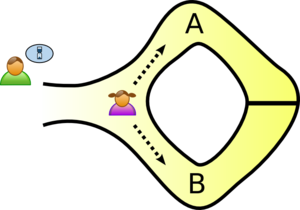
\includegraphics[width=\textwidth]{images/zkp1.png}
        \end{subfigure}
        \hspace{0.25cm}
        \begin{subfigure}{0.25\textwidth}
            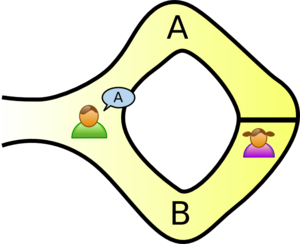
\includegraphics[width=\textwidth]{images/zkp2.png}
        \end{subfigure}
        \hspace{0.25cm}
        \begin{subfigure}{0.25\textwidth}
            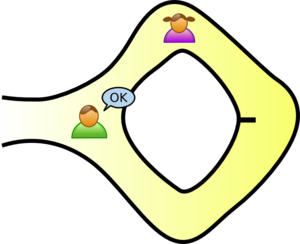
\includegraphics[width=\textwidth]{images/zkp3.png}
        \end{subfigure}
        \caption[Jama Ali Babe.]{Igra Ane in Bojana v jami Ali Babe. Vir slike Wikipedia~\cite{zkp}.}
        \label{fig:alibaba}
    \end{figure}
\end{primer}

\subsubsection{Dokazi znanja brez razkritja znanja}
Za namene kriptografije so pogosto zanimivi dokazi brez razkritja znanja. Da vzpostavimo zaupanje
(npr.\ med dvema strankama, ki se ne poznata), pa ne želimo samo, da ena stranka dokaže obstoj neke
skrivnosti, ampak tudi, da to skrivnost dejansko pozna. To je osnovna ideja \textit{dokazov znanja
brez razkritja znanja} (angl.\ \textit{zero-knowledge proofs of knowledge}).

Odličen primer tovrstnega dokaza je dokaz znanja o tem, da poznamo diskretni logaritem dane vrednosti.
Ta dokaz ima neposredno uporabo v kriptografiji, saj tako lahko dokažemo, da nek javni ključ res
pripada nam. Denimo, da smo ustvarili par ključev $(I, s)$, kjer je $I = g^s$ javni ključ, $s$ pa
zasebni ključ. Če nam preverjevalec predloži vrednost $I = g^s$, mi pa ga uspemo prepričati, da poznamo
vrednost $s$, potem je to dovolj, da preverjevalec verjame, da je $I$ res naš javni ključ (razen z
zanemarljivo verjetnostjo).

Dokazovanje dejstva, da nek javni ključ res pripada nam prek interaktivnega protokola ima veliko
uporabno vrednost. Tovrstne dokaze imenujemo \textit{identifikacijski protokoli} oz.\ sheme.

\begin{primer}[Schnorrov identifikacijski protokol]
    En izmed najenostavnejših protokolov za dokaz znanja brez razkritja znanja je Schnorrov
    protokol~\cite{schnorr1989sig}. Tesno je povezan s Schnorrovim podpisom, ki ga bomo spoznali v
    naslednjem razdelku. Protokol poteka med dokazovalcem, ki želi dokazati preverjevalcu, da
    pozna diskretni logaritem dane vrednosti, in preverjevalcem, ki želi to preveriti.

    Pred začetkom se morata strinjati o ciklični grupi $G$ reda $q$, ki jo generira element $g$. Ta
    grupa predstavlja ogrodje za protokol. Prav tako je obema na voljo javni podatek
    $$
    I = g^s \in G.
    $$
    Cilj dokazovalca je, da preverjevalca prepriča, da pozna vrednost $s \in \Z_q$, ne da bi mu
    o njej razkril karkoli drugega. Protokol poteka v več korakih:
    \begin{enumerate}
        \item \textbf{Zaveza:}
            Dokazovalec si enakomerno naključno izbere vrednost $r \in \Z_q$ in izračuna
            $$
            X = g^r \in G.
            $$
            To vrednost pošlje preverjevalcu.
        \item \textbf{Izziv:}
            Preverjevalec si izbere naključno vrednost $e \in \Z_q$ in jo pošlje dokazovalcu.
        \item \textbf{Odgovor:}
            Dokazovalec izračuna odgovor
            $$
            y = r + es
            $$
            in ga pošlje preverjevalcu.
        \item \textbf{Preverjanje:}
            Preverjevalec preveri, če velja
            $$
            g^y = X \cdot I^e.
            $$
            Če enakost drži, preverjevalec verjame, da dokazovalec pozna vrednost $s$, saj je
            $$
            g^y = g^{r + es} = g^r \cdot g^{es} = X \cdot I^e.
            $$
    \end{enumerate}
    Varnost protokola temelji na težavnosti problema diskretnega logaritma in pa na dejstvu, da je
    izziv določen po zavezi. Zato dokazovalec ne more izračunati prepričjivega odgovora, preden
    dobi izziv. Bolj formalno bomo varnost dokazali pri dokazu varnosti Schnorrovega podpisa v
    razdelku~\ref{sec:schnorr-sec}.
\end{primer}

\subsubsection{Fiat-Shamirjeva hevristika}
\label{sec:fiat-shamir}
Dokazi znanja brez razkritja znanja so torej odlično splošno orodje, s katerim se lahko prepričamo
o identiteti sogovornika, ne da bi ta moral razkriti skrivni ključ. V praksi pa je težava, da so
taki protokoli interaktivni, kar pomeni, da zahtevajo neposredno komunikacijo med dokazovalcem in
preverjevalcem. Ta komunikacija je zamudna in draga.

Fiat in Shamir sta leta $1987$~\cite{fiat1987heuristic} predlagala način, kako lahko interaktivne
dokaze znanja spremenimo v neinteraktivne. Osnovna ideja je, da namesto preverjevalca, breme izbire
izziva prenesemo na slučajnega oraklja, do katerega imata dostop tako dokazovalec kot preverjevalec.
Hevristika torej deluje samo v modelu slučajnega oraklja.

\begin{primer}[Schnorrova shema in Fiat-Shamirjeva hevristika]
\label{primer:fiat-shamir}
    S pomočjo Fiat-Shamirjeve hevristike lahko Schnorrovo identifikacijsko shemo spremenimo v
    neinteraktivno, kar praktično neposredno privede do Schnorrovega podpisa, ki ga bomo spoznali
    v naslednjem razdelku.

    Glavna ideja je, da se znebimo preverjevalčevega izziva. Namesto tega dokazovalec uporabi
    oraklja $H$, da pridobi zgostitev iz zaveze $X$ in sporočila $m$, ki ga želi podpisati (ta
    korak tudi veže sporočilo na podpis):
    $$
    e = H(\text{enc}(X) || m),
    $$
    kjer ">$||$"< označuje stikanje nizov. Na podlagi te zgostitve dokazovalec izračuna odgovor
    $y = r + es$ in ga pošlje preverjevalcu skupaj z vrednostjo $X$ in $e$. Preverjevalec ima sedaj
    dovolj podatkov, da tudi sam izračuna vrednost zgostitve in preveri enakost.

    Fiat-Shamirjeva hevristika tu ohranja varnost, saj dokazovalec še vedno ne more izračunati
    prepričljivega odgovora, preden izračuna zavezo (razen, če najde trk v $H$). Nekaj bitov
    varnosti se vseeno izgubi, ker napadalcu ni potrebno več čakati na odgovore, pač pa lahko izračuna
    poljubno mnogo zgostitev. Ob dovolj velikih parametrih to dejstvo ne predstavlja težav. Varnost bomo
    dokazali v razdelku~\ref{sec:schnorr-sec}.
\end{primer}
